\documentclass{standalone}
\usepackage{pgfplots}
\usetikzlibrary {arrows.meta}
\pgfplotsset{width=7cm,compat=1.8}
\begin{document}
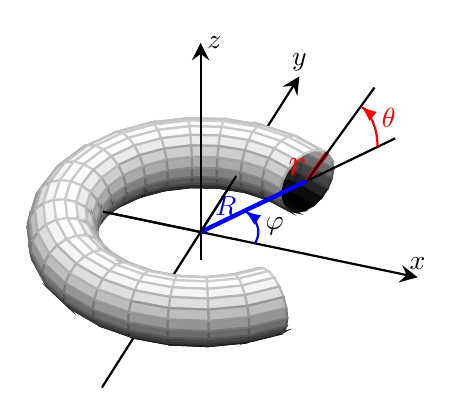
\begin{tikzpicture}[scale=2]
    \begin{axis}[axis equal image,
        axis lines=middle,
        xmax=20,ymax=25,zmax=20, ymin=-25,
        ticks=none,
        clip bounding box=upper bound,
        colormap/blackwhite,
        view={20}{35}
        ]

        \addplot3[domain=0:360,y domain=60:320, samples=20,surf,z buffer=sort]
            ({(12 + 3 * cos(x)) * cos(y)} ,
            {(12 + 3 * cos(x)) * sin(y)},
            {3 * sin(x)});
        %use axis coordinate system to draw the radii
        \draw [thick, blue] (axis cs: 0,0,0) -- node [scale=0.5, yshift=-0.0em, xshift=-1em]{$R$} (axis cs: {12*cos(60)},{12*sin(60)},0);
        \draw [thick, red] (axis cs: {12*cos(60)},{12*sin(60)},0) -- node [scale=0.7, xshift=-0.5em]{$r$}(axis cs: {(12 + 3*cos(40))*cos(60)},{(12+3*cos(40))*sin(60)}, {3*sin(40)});
        \node at (axis cs: 20,0,0) [scale=0.5, yshift=0.5em]{$x$};
        %use axis coordinate system to draw FAKE x, y and z axes
        \node [scale=0.5, xshift=0.5em] at (axis cs: 0,0,20){$z$};
        \draw (axis cs: 0,0,0) -- (axis cs: 0, 0 ,15);
        % \draw [-latex]  (axis cs: 0,-15,0) --
        %  node [pos=0.9, xshift=-1em, yshift=0.5em]{$y$}(axis cs: 0,-25,0);
        \node [scale=0.5, yshift=0.5em] at (axis cs: 0,25,0){$y$};
        \draw (axis cs: 0,0,0) -- (axis cs: 0,9,0);
        \draw (axis cs: 0,0,0) -- (axis cs: -9,0,0);
        \addplot3[domain=0:60, blue, samples y=1, -{Latex[length=1mm]}]({5*cos(x)},{5*sin(x)},{0});
        \node [scale=0.5, yshift=-0.5em] at (axis cs: 5,5,0){$\varphi$};
        \draw [thin] (axis cs: {12*cos(60)},{12*sin(60)},0) -- (axis cs: {(12 + 10*cos(40))*cos(60)},{(12+10*cos(40))*sin(60)}, {10*sin(40)});
        \draw [thin] (axis cs: {12*cos(60)},{12*sin(60)},0) -- (axis cs: {(12 + 10*cos(0))*cos(60)},{(12+10*cos(0))*sin(60)}, {10*sin(0)});
        \addplot3[domain=0:40, red, samples y=1, -{Latex[length=1mm]}]({(12 + 8*cos(x))*cos(60)},{(12+8*cos(x))*sin(60)}, {8*sin(x)});
        \node [scale=0.5, red, yshift=-0.5em] at (axis cs: 9.7,21,2){$\theta$};



    \end{axis}
\end{tikzpicture} 
\end{document}